\cleardoublepage
\clearpage{}

%[Lo que va en el índice]{Lo que va en el documento}
\chapter[Metodología de trabajo]{Metodología de trabajo}
\section{Metodología de trabajo seguida en el documento}
Desde el comienzo del trabajo se ha seguido una especie de metodología ágil. Cada semana o cada dos semanas se celebraba una reunión con el tutor, estas reuniones se por norma general tenían lugar a través de Google Meet. En dichas reuniones exponía el trabajo que había realizado tras la reunión anterior, se resolvían las dudas que habían ido surgido y se proponían una serie de objetivos que, deseablemente había que trabajar de cara a la siguiente reunión. Gracias a seguir esta forma de organización, logramos avanzar en el proyecto, que a principio parecía inabarcable pero no resultó ser así. \\

Con el fin de tener un registro de como iba avanzando la memoria, creamos un repositorio en \href{http://www.github.com}{\textit{Github}}. Este repositorio estaba enlazado con el proyecto alojado en \href{http://www.overleaf.com}{\textit{Overleaf}} y al final de casa sesión de trabajo se subían los cambios. Desafortunadamente esta idea surgió tarde y las primeras versiones del documento no se encuentran registradas en el repositorio.\\

En referencia a la búsqueda de información el objetivo era primar la información de calidad, para ello siempre hemos tratado de acudir a documentaciones oficiales (si estaban disponibles) o directamente consultar bibliografía de prestigio. En caso de que esto no fuera posible, el siguiente paso era buscar información de empresas relacionadas con la cuestión a tratar (por ejemplo: Ext4 la documentación oficial disponible es muy escueta, mientras que la información disponible en la página de Fedora es bastante completa.) y por último lugar buscar en \textit{papers} ya que en algunos casos hay información muy buena, pero es complicado sacar información de este tipo de documentos por los motivos que se explicaron en la sección \ref{estado}.

\section{Metodología de los experimentos}
El objetivo de este trabajo requiere comparar el rendimiento de Btrfs, Ext4 y XFS en un único disco. Para realizar la comparativa de rendimiento, uno debería plantearse el uso de distintas herramientas de \textit{benchmarking} que sean capaces de mostrar el comportamiento de los sistemas de archivos bajo una determinada carga. Para este caso específico diremos que existen dos tipos de \textit{benchmarks}. \\

Por un lado tenemos \textit{benchmarks} reales (por ejemplo medir el rendimiento de una tarjeta gráfica utilizando un videojuego). El uso de este tipo de \textit{benchmarks} tiene aspectos positivos, pero resulta difícil encontrar aplicaciones suficientemente representativas que engloben el funcionamiento de un sistema de archivos en todas la situaciones.\\

Por otro lado tenemos los \textit{benchmarks} sintéticos. Son programas artificiales que no realizan ningún trabajo real y útil. Las operaciones realizadas por estos \textit{benchmarks} se eligen cuidadosamente para que coincidan con las operaciones que realizaría otro tipo de programas. El objetivo es que las operaciones que realiza el \textit{benchmark} sean lo mas similares posible para así poder exportar los resultados al mundo real \cite{lilja_2000}.\\

La combinación de ambos tipos de \textit{benchmarks} para la medición de rendimiento de E/S del sistema de archivos producirá un resultado más representativo en lugar de depender únicamente de uno de los dos tipos de herramientas. Este proyecto hace uso tanto de \textit{benchmarks} sintéticos elaborados con \textit{Filebench} como de aplicaciones reales para las medidas.

\section{Entorno de pruebas y repetición de experimentos}
El estado del sistema a la hora de ejecutar las pruebas puede influir en los resultados. Por poner un ejemplo, tal y como señala Avishay Traeger \cite{traeger} el estado de la caché a la hora de ejecutar un test es determinante. No está del todo claro la metodología a seguir en estos casos, por un lado en un entorno real la caché no estaría completamente fría\footnote{Caché fría: Cuando la caché está vacía o contiene datos irrelevantes, esta situación conlleva hacer lecturas desde memoria principal.}. Por otro lado un \textit{benchmark} que accede a demasiados datos que se encuentran almacenados en caché también es poco realista. Si deseamos resultados de caché fría, habrá que desmontar el sistema de archivos tras cada ejecución para asegurar que la caché queda limpia tanto la del disco como la de la CPU \cite{traeger}. En nuestro caso, montaremos y desmontaremos el sistema de archivos entre pruebas para asegurar unos resultados fiables.\\

Haciendo referencia de nuevo a Avishay Traeger bajo su criterio existen cuatro pautas importantes \cite{traeger} a la hora de ejecutar un \textit{benchmark}: 

\begin{enumerate}
    \item Asegurar que cada vez que se ejecuta un \textit{benchmark} sea bajo idéntica configuración.
    \item Cada prueba debe realizarse varias veces para garantizar la precisión. Los niveles de confianza deben utilizarse para determinar el número adecuado de ejecuciones.
    \item Las pruebas se deben realizar durante un periodo de tiempo lo suficientemente largo.
    \item El proceso de \textit{benchmarking} debe automatizarse utilizando scripts u otras herramientas de automatización.
\end{enumerate}

Nos centraremos en la segunda pauta ya que puede ser la menos intuitiva de entender. Nos interesa que el número de mediciones sea el mínimo sin que esto afecte a la calidad de los resultados. Basándonos en la fórmula de los intervalos de confianza determinaremos cuantas medidas son necesarias para producir un intervalo de una anchura específica \cite{lilja_2000}. \\

Supongamos que queremos definir un intervalo de confianza para $\Bar{x}$ así que hay una probabilidad de $1-\alpha$ de que el valor actual de $x$ esté contenido en el intervalo  $$
\left(c_{1}, c_{2}\right)=((1-e) \bar{x},(1+e) \bar{x})
$$ 
Entonces tenemos que 
$$
c_{1}=(1-e) \bar{x}=\bar{x}-z_{1-\alpha / 2} \frac{s}{\sqrt{n}}
$$
$$
c_{2}=(1+e) \bar{x}=\bar{x}+z_{1-\alpha / 2} \frac{s}{\sqrt{n}}
$$
Como ambos intervalos son simétricos podemos utilizar cualquiera de las dos ecuaciones para determinar que:
$$
z_{1-\alpha / 2} \frac{s}{\sqrt{n}}=\bar{x} e
$$
Despejando $n$ obtendríamos
$$
n=\left(\frac{z_{1-\alpha / 2} s}{e \bar{x}}\right)^{2}
$$ 

Para determinar el número de mediciones se requiere una estimación de la desviación estándar ($s$). Sin embargo, no podemos saber acerca de la desviación hasta que no hagamos algunas mediciones. Por tanto, el procedimiento consiste en realizar un número relativamente pequeño de mediciones para realizar una estimación de la desviación \cite{lilja_2000}. \\ 

Para el cálculo del número de medidas necesarias y tomando como guía una de las cuatro pautas de Avishay Traeger, dicho cálculo se realizará, en la medida de lo posible, automáticamente. El código de dicho programa es el siguiente:  

\section{Test Anova}
Una vez se hayan ejecutado las pruebas el número de veces necesarias, se podrá observar que los resultados entre las alternativas varían. Esta variación podría ser debida al cambio de factor en la alternativa o podría ser solo ruido en la medición. Debido a ello se hará uso del test anova (\textit{\textbf{An}alisys \textbf{o}f \textbf{Va}riance})\\

El análisis de varianza es una técnica para dividir la variación de unas mediciones y convertirla en mediciones significativas. Este tipo de análisis asume que los errores en las mediciones de las distintas alternativas son independientes y siguen una distribución gaussiana (distibución normal). Se supone que la varianza del error es la misma para todas las alternativas. El test Anova divide la variación en dos, por un lado la variación causada por los errores en las mediciones y por otro lado la variación entre sistemas. El objetivo es determinar si la variación ente sistemas se debe a la diferencia real entre sistemas o simplemente es debido a error en la medición. \cite{lilja_2000} \\

¿Las diferencias entre las medidas observadas para las alternativas se deben a diferencias reales entre las alternativas, o se deben simplemente a errores de medición? \cite{lilja_2000} \\

Para resolver esta cuestión, necesitamos hacer $n$ mediciones en cada una de las $k$ alternativas. Según Lilja \cite{lilja_2000} es conveniente organizar las mediciones en una tabla cómo la siguiente. 
 
\begin{figure}[H]
    \centering
    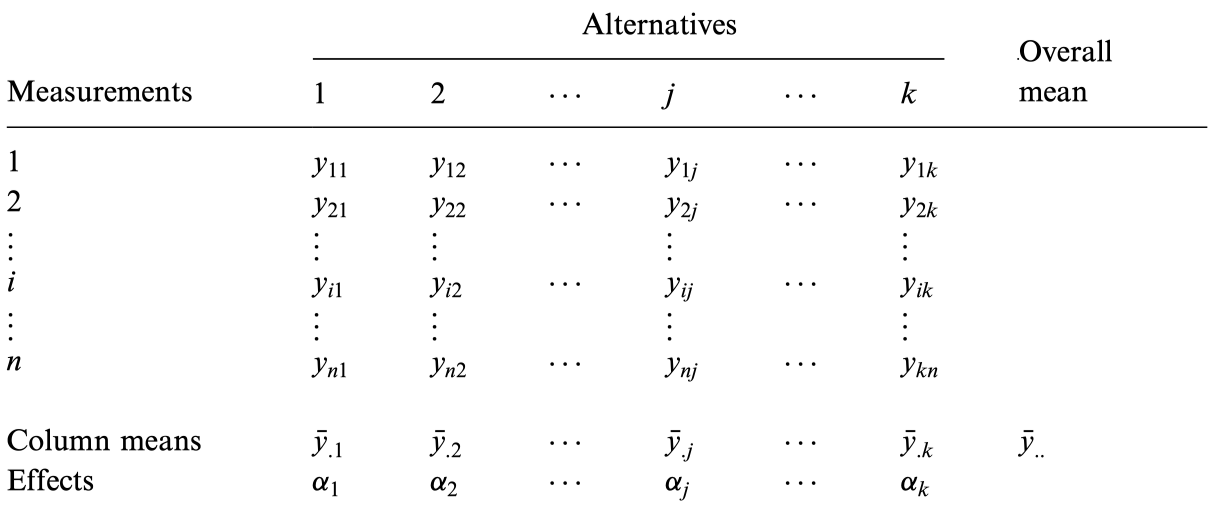
\includegraphics[scale=0.6]{doc/assets/images/Capitulo3/lilja_recommend.png}
    \caption{Como se deben ordenar las mediciones para facilitar los cálculos del test Anova \cite{lilja_2000}}
    \label{fig:Anova_liljal}
\end{figure}

Dónde $y_{ij}s$ es la i-ésima medida de la j-ésima alternativa. La fila de la media de las columnas se denomina $\Bar{y}_{.j}$ y se calcula como $
\bar{y}_{. j}=\frac{\sum_{i=1}^{n} y_{i j}}{n}
$. La media total $\Bar{y}_{..}$ es la media de todas las medidas realizadas en todas las alternativas cuya fórmula sería $$
\bar{y}_{. .}=\frac{\sum_{j=1}^{n} \sum_{i=1}^{n} y_{i j}}{k n}
$$.

Es útil descomponer cada medida $y_{ij}$ como la suma de de todas las medias de la alternativa $j$, $\bar{y}_{.j}$ y un valor $e_{ij}$ que representa la desviación de la medición respecto a la media. Por lo que partiendo de este enunciado la ecuación resultante es: $$y_{ij}=\bar{y}_{.j} + e_{ij}$$.

Podemos extender este razonamiento para representar la fila de medias $\bar{y}_{ij}$ como la suma de la  media total $\bar{y}_{..}$ y la desviación de la fila de las medias $\alpha_j$. Como resultado obtenemos: $$
y_{i j}=\bar{y}_{. .}+\alpha_{j}+e_{i j}
$$

Expresar las medidas de esta forma nos permite dividir la variación de todas las medidas en dos componentes separados. Por un lado la variación provocada por los efectos de las alternativas y por otro lado la variación debida a los errores. Respecto a la variación debida a los efectos de las alternativas la cual no debemos confundirla con la varianza, comúnmente se denomina \textit{SSA} y es calculada de la siguiente forma :  $$S S A=n \sum_{j=1}^{k}\left(\bar{y}_{. j}-\bar{y}_{. .}\right)^{2}$$. 

De forma similar la variación debida a errores se denota como \textit{SSE}. Calculada como la sumatoria del cuadrado de las diferencias entre las medidas individuales y y su correspondiente media total. De este modo tenemos que:  $$S S E=\sum_{j=1}^{k} \sum_{i=1}^{n}\left(y_{i j}-\bar{y}_{. j}\right)^{2}$$ 

Finalmente, la varianza residual se calcula como:
$$
S S T=\sum_{j=1}^{k} \sum_{i=1}^{n}\left(y_{i j}-\bar{y}_{..}\right)^{2}
$$

De todo esto podemos deducir que $$S S T= S S A + S S E$$

El objetivo es contrastar la hipótesis de que el factor no influye sobre los resultados. Si esto es así el resultado de calcular $F_{exp}$ debería ser una muestra de una distribucion F de Snedecor.

$$
F_{e x p} = \frac{\operatorname{SSA} /\left(k-1\right)}{\operatorname{SSE} /\left (k(n-1)\right) } \sim F_{k-1,k(n-1)}
$$
\\
La prueba estadística que ha demostrado ser adecuada para este tipo de comparativas es el test-F. Este test, que se basa en la distribución F de Snedecor, se utiliza para comprobar si dos varianzas son significativamente diferentes. Dado que el estadístico F se calcula como el cociente de dos varianzas, los valores cercanos a 1 indicarán que probablemente no existe ninguna diferencia significativa.\\

Las estimaciones de las varianzas de $SSA$ y $SSE$ se hallan calculando sus correspondientes valores de \textit{mean-square}. El \textit{mean-square} es simplemente la variación total del componente dividida por el número de grados de libertad de ese componente. Dado que se comparan $k$ alternativas, hay $k-1$ grados de libertad en $SSA$. Por lo que, la estimación de la varianza es: $$
s_{\mathrm{a}}^{2}=\frac{S S A}{k-1}
$$

De forma similar ocurre con $SSE$ como cada una de las alternativas tiene n-mediciones, cada alternativa tiene $n-1$ grados de libertad. Por lo tanto, el número total de grados de libertad para $SSE$ es $kn-1$, ya que hay k alternativas. La estimación de la varianza del error es entonces: 
$$
s_{\mathrm{a}}^{2}=\frac{S S E}{k(n-1)}
$$

Finalmente el estadístico $F$ para este test es calculado de la siguiente manera: $$
F=\frac{s_{\mathrm{a}}^{2}}{s_{\mathrm{e}}^{2}}
$$

Dado que el estadístico $F$ es calculado como el cociente de dos varianza necesitará de dos valores para los grados de libertad. Si el valor de F calculado es mayor que el valor $F_{[1-\alpha ;(k-1), k(n-1)]}$ obtenido de la tabla, diremos que la variación causada entre las alternativas es mayor que la causada por los errores en un nivel de confianza de $1-\alpha$.



\section{Máquina de pruebas}
Los experimentos fueron ejecutados en una máquina convencional con un procesador AMD con una frecuencia de reloj de 3.5 GHz. Ubuntu 16.04.7 fue la versión del sistema operativo en el que se ejecutaron las pruebas. El sistema tenía 2 discos, en un disco SSD se encontraba el sistema operativo y las herramientas de \textit{benchmark} y el disco HDD se utilizaba exclusivamente para el montaje de los sistemas de archivos. La tabla siguiente muestra todos los detalles sobre el hardware y software utilizado.
\begin{table}[h]
    \centering
    \begin{tabular}{|l|l|}
    \hline
        Componente & Modelo \\ \hline\hline
        CPU & AMD Ryzen 3 1300X @ 3.5 GHz Quad-Core \\ \hline
        Memoria & Crucial CT8G4DFS824A. 8 GB DDR4 2400 MHz CL17 \\ \hline
        Placa Base & ASUS EX-A320M \\ \hline
        SSD del Sistema & Kingston A400 SSD SATA3 \\ \hline
        HDD de Pruebas & Seagate Barracuda ST500DM002-1BD14 500GB \\ \hline
    \end{tabular}
    \caption{Especificaciones Hardware}
\label{table:1}
\end{table}

\begin{table}[H]
    \centering
    \begin{tabular}{|l|l|}
    \hline
        Software & Versión \\ \hline\hline
        Ubuntu 18.04.5 LTS & Kernel GNU/Linux 5.4.0-42-generic x86\_64 \\ \hline
        Filebench & 1.5-alpha3 \\ \hline
        KownSeq & XXXXXXXXXXX \\ \hline
        iozone & XXXXXXXXXXXX \\ \hline
        R & xxxxxxxxxxxxx \\ \hline
    \end{tabular}
    \caption{Especificaciones Software}
\label{table:2}
\end{table}



\section{Herramientas de \textit{benchmarking} y metodología}
\subsection{Iozone}
Iozone en general es utilizado para medir el rendimiento del sistema de archivos, utilizando distintos tipos de pruebas. Utilizamos esta herramienta para medir el rendimiento en operaciones de lectura, escritura, re-lectura, re-escritura, lectura aleatoria y escritura aleatoria. Se han seleccionado estas operaciones debido a que, son operaciones que son ejecutadas por las aplicaciones, bajo cualquier tipo de sistema de archivos. Iozone es una suite ampliamente extendida en el mundo de los \textit{benchmarks}, probablemente debido a su variedad de ajustes y es por ello por lo que la vamos a utilizar.

\subsection{Filebench}
Utilizaremos esta herramienta principalmente por disponer de un lenguaje para modelar carga. Es decir, utilizaremos Filebench WML para crear benchmarks sintéticos. El objetivo es crear un benchmark desde 0, que se simule un uso real del disco por parte de una aplicación genérica o un usuario genérico. 
%\subsection{iowatcher}

\subsection{KnowSeq}
KnowSeq es una herramienta que permite procesar y extraer biomarcadores relevantes, así como evaluarlos mediante enfoques de Machine Learning. El objetivo de KnowSeq es la extracción de conocimiento biológico a partir de biomarcadores. \\

En nuestro caso concreto utilizaremos una parte del cauce del programa. Este cauce se encarga del tratamiento de los datos en crudo. Este proceso consiste en extraer un conjunto de archivos provenientes de los datos en bruto alojados en el repositorio del programa.Partimos de unos archivos SRA y el objetivo es procesarlos para obtener unos ficheros llamados \textit{count files}. La transformación de un archivo SRA a \textit{count file} no es directa, si no que existen pasos intermedios que generan por tanto archivos intermedios. Estos ficheros se denominan \textit{FASTQ, BAM y SAM Files} y son archivos muy pesados (del orden de 10-15 GB). KnowSeq conforme va generando los FASTQ, BAM, SAM Files los va organizando en carpetas, es decir mueve archivos pesados, por lo que durante el proceso se hacen operaciones muy pesadas en el sistema de archivos.\\

Para esta prueba utilizaremos series relativas al Covid-19. Knowseq en su repositorio tiene datos de 90 pacientes, pero desafortunadamente se utilizarán sólo datos de 20 de ellos, ya que al ser archivos tan pesados necesitaríamos una cantidad de espacio que no disponemos y el tiempo de procesamiento es demasiado alto (~2h/paciente). Además al realizar las mismas operaciones sobre archivos aunque sean distintos pacientes, hacen que los resultados sean fácilmente exportables a un número mayor de pacientes. 

\section{Instalación de paquetes}
\subsection{IOzone}
\subsection{IOwatcher}
\subsection{KnowSeq}
\subsection{Filebecnh}